% Options for packages loaded elsewhere
\PassOptionsToPackage{unicode}{hyperref}
\PassOptionsToPackage{hyphens}{url}
%
\documentclass[
]{article}
\usepackage{lmodern}
\usepackage{amssymb,amsmath}
\usepackage{ifxetex,ifluatex}
\ifnum 0\ifxetex 1\fi\ifluatex 1\fi=0 % if pdftex
  \usepackage[T1]{fontenc}
  \usepackage[utf8]{inputenc}
  \usepackage{textcomp} % provide euro and other symbols
\else % if luatex or xetex
  \usepackage{unicode-math}
  \defaultfontfeatures{Scale=MatchLowercase}
  \defaultfontfeatures[\rmfamily]{Ligatures=TeX,Scale=1}
\fi
% Use upquote if available, for straight quotes in verbatim environments
\IfFileExists{upquote.sty}{\usepackage{upquote}}{}
\IfFileExists{microtype.sty}{% use microtype if available
  \usepackage[]{microtype}
  \UseMicrotypeSet[protrusion]{basicmath} % disable protrusion for tt fonts
}{}
\makeatletter
\@ifundefined{KOMAClassName}{% if non-KOMA class
  \IfFileExists{parskip.sty}{%
    \usepackage{parskip}
  }{% else
    \setlength{\parindent}{0pt}
    \setlength{\parskip}{6pt plus 2pt minus 1pt}}
}{% if KOMA class
  \KOMAoptions{parskip=half}}
\makeatother
\usepackage{xcolor}
\IfFileExists{xurl.sty}{\usepackage{xurl}}{} % add URL line breaks if available
\IfFileExists{bookmark.sty}{\usepackage{bookmark}}{\usepackage{hyperref}}
\hypersetup{
  pdftitle={Project 4},
  pdfauthor={Anton Stråhle \& Max Sjödin},
  hidelinks,
  pdfcreator={LaTeX via pandoc}}
\urlstyle{same} % disable monospaced font for URLs
\usepackage[margin=1cm]{geometry}
\usepackage{longtable,booktabs}
% Correct order of tables after \paragraph or \subparagraph
\usepackage{etoolbox}
\makeatletter
\patchcmd\longtable{\par}{\if@noskipsec\mbox{}\fi\par}{}{}
\makeatother
% Allow footnotes in longtable head/foot
\IfFileExists{footnotehyper.sty}{\usepackage{footnotehyper}}{\usepackage{footnote}}
\makesavenoteenv{longtable}
\usepackage{graphicx,grffile}
\makeatletter
\def\maxwidth{\ifdim\Gin@nat@width>\linewidth\linewidth\else\Gin@nat@width\fi}
\def\maxheight{\ifdim\Gin@nat@height>\textheight\textheight\else\Gin@nat@height\fi}
\makeatother
% Scale images if necessary, so that they will not overflow the page
% margins by default, and it is still possible to overwrite the defaults
% using explicit options in \includegraphics[width, height, ...]{}
\setkeys{Gin}{width=\maxwidth,height=\maxheight,keepaspectratio}
% Set default figure placement to htbp
\makeatletter
\def\fps@figure{htbp}
\makeatother
\setlength{\emergencystretch}{3em} % prevent overfull lines
\providecommand{\tightlist}{%
  \setlength{\itemsep}{0pt}\setlength{\parskip}{0pt}}
\setcounter{secnumdepth}{-\maxdimen} % remove section numbering

\title{Project 4}
\author{Anton Stråhle \& Max Sjödin}
\date{28 december 2020}

\begin{document}
\maketitle

\hypertarget{introduction}{%
\section{Introduction}\label{introduction}}

This is a project for the course MT7038 which was given during the fall
of 2020. In the project we'll examine some basic methods for binary
classification on a granular level and then proceed with a more in depth
analysis and discussion for those that seem to perform best. The methods
that we will initially test are SVM, KNN and Decision Trees.

\hypertarget{data}{%
\section{Data}\label{data}}

We picked the \texttt{Occupancy\ Detection} data set as we wanted to
work with a binary classification problem as this would allow us to
apply most of the methodologies discussed throughout the course. As
there are quite a few different binary data sets at UCI we specifically
chose our data set as it had a sizeable number of instances as well as
few, but intuitivley explanatory, features.

\hypertarget{attributes}{%
\subsection{Attributes}\label{attributes}}

The data \texttt{Occupancy\ Detection} data set includes snapshots of a
specific room every minute throughout the course of a few weeks. The aim
is to classify the current \texttt{Occupancy} of the room using the five
features, \texttt{Temperature}, \texttt{CO2}, \texttt{Humidity},
\texttt{HumidityRatio} and \texttt{Light}, which are observed each
minute. The first three features are quite self-explanatory but the two
final ones could use some clarification. The \texttt{Light} in the room
is the light intensity, measured in Lux whilst the
\texttt{HumidityRatio} is vaguely described as a ``derived quantity from
temperature and relative humidity, in kgwater-vapor/kg-air''.

\hypertarget{exploration}{%
\subsection{Exploration}\label{exploration}}

From a quick overview we see that the data set is quite unbalanced.

\begin{longtable}[]{@{}lrrrrrrrrrrrrr@{}}
\caption{Unoccupied}\tabularnewline
\toprule
\begin{minipage}[b]{0.08\columnwidth}\raggedright
\strut
\end{minipage} & \begin{minipage}[b]{0.03\columnwidth}\raggedleft
vars\strut
\end{minipage} & \begin{minipage}[b]{0.03\columnwidth}\raggedleft
n\strut
\end{minipage} & \begin{minipage}[b]{0.05\columnwidth}\raggedleft
mean\strut
\end{minipage} & \begin{minipage}[b]{0.05\columnwidth}\raggedleft
sd\strut
\end{minipage} & \begin{minipage}[b]{0.05\columnwidth}\raggedleft
median\strut
\end{minipage} & \begin{minipage}[b]{0.05\columnwidth}\raggedleft
trimmed\strut
\end{minipage} & \begin{minipage}[b]{0.05\columnwidth}\raggedleft
mad\strut
\end{minipage} & \begin{minipage}[b]{0.05\columnwidth}\raggedleft
min\strut
\end{minipage} & \begin{minipage}[b]{0.05\columnwidth}\raggedleft
max\strut
\end{minipage} & \begin{minipage}[b]{0.05\columnwidth}\raggedleft
range\strut
\end{minipage} & \begin{minipage}[b]{0.04\columnwidth}\raggedleft
skew\strut
\end{minipage} & \begin{minipage}[b]{0.05\columnwidth}\raggedleft
kurtosis\strut
\end{minipage} & \begin{minipage}[b]{0.03\columnwidth}\raggedleft
se\strut
\end{minipage}\tabularnewline
\midrule
\endfirsthead
\toprule
\begin{minipage}[b]{0.08\columnwidth}\raggedright
\strut
\end{minipage} & \begin{minipage}[b]{0.03\columnwidth}\raggedleft
vars\strut
\end{minipage} & \begin{minipage}[b]{0.03\columnwidth}\raggedleft
n\strut
\end{minipage} & \begin{minipage}[b]{0.05\columnwidth}\raggedleft
mean\strut
\end{minipage} & \begin{minipage}[b]{0.05\columnwidth}\raggedleft
sd\strut
\end{minipage} & \begin{minipage}[b]{0.05\columnwidth}\raggedleft
median\strut
\end{minipage} & \begin{minipage}[b]{0.05\columnwidth}\raggedleft
trimmed\strut
\end{minipage} & \begin{minipage}[b]{0.05\columnwidth}\raggedleft
mad\strut
\end{minipage} & \begin{minipage}[b]{0.05\columnwidth}\raggedleft
min\strut
\end{minipage} & \begin{minipage}[b]{0.05\columnwidth}\raggedleft
max\strut
\end{minipage} & \begin{minipage}[b]{0.05\columnwidth}\raggedleft
range\strut
\end{minipage} & \begin{minipage}[b]{0.04\columnwidth}\raggedleft
skew\strut
\end{minipage} & \begin{minipage}[b]{0.05\columnwidth}\raggedleft
kurtosis\strut
\end{minipage} & \begin{minipage}[b]{0.03\columnwidth}\raggedleft
se\strut
\end{minipage}\tabularnewline
\midrule
\endhead
\begin{minipage}[t]{0.08\columnwidth}\raggedright
Temperature\strut
\end{minipage} & \begin{minipage}[t]{0.03\columnwidth}\raggedleft
1\strut
\end{minipage} & \begin{minipage}[t]{0.03\columnwidth}\raggedleft
15810\strut
\end{minipage} & \begin{minipage}[t]{0.05\columnwidth}\raggedleft
20.585\strut
\end{minipage} & \begin{minipage}[t]{0.05\columnwidth}\raggedleft
0.895\strut
\end{minipage} & \begin{minipage}[t]{0.05\columnwidth}\raggedleft
20.500\strut
\end{minipage} & \begin{minipage}[t]{0.05\columnwidth}\raggedleft
20.488\strut
\end{minipage} & \begin{minipage}[t]{0.05\columnwidth}\raggedleft
0.741\strut
\end{minipage} & \begin{minipage}[t]{0.05\columnwidth}\raggedleft
19.000\strut
\end{minipage} & \begin{minipage}[t]{0.05\columnwidth}\raggedleft
24.390\strut
\end{minipage} & \begin{minipage}[t]{0.05\columnwidth}\raggedleft
5.390\strut
\end{minipage} & \begin{minipage}[t]{0.04\columnwidth}\raggedleft
1.325\strut
\end{minipage} & \begin{minipage}[t]{0.05\columnwidth}\raggedleft
2.757\strut
\end{minipage} & \begin{minipage}[t]{0.03\columnwidth}\raggedleft
0.007\strut
\end{minipage}\tabularnewline
\begin{minipage}[t]{0.08\columnwidth}\raggedright
Humidity\strut
\end{minipage} & \begin{minipage}[t]{0.03\columnwidth}\raggedleft
2\strut
\end{minipage} & \begin{minipage}[t]{0.03\columnwidth}\raggedleft
15810\strut
\end{minipage} & \begin{minipage}[t]{0.05\columnwidth}\raggedleft
27.530\strut
\end{minipage} & \begin{minipage}[t]{0.05\columnwidth}\raggedleft
5.119\strut
\end{minipage} & \begin{minipage}[t]{0.05\columnwidth}\raggedleft
27.150\strut
\end{minipage} & \begin{minipage}[t]{0.05\columnwidth}\raggedleft
27.556\strut
\end{minipage} & \begin{minipage}[t]{0.05\columnwidth}\raggedleft
5.411\strut
\end{minipage} & \begin{minipage}[t]{0.05\columnwidth}\raggedleft
16.745\strut
\end{minipage} & \begin{minipage}[t]{0.05\columnwidth}\raggedleft
39.500\strut
\end{minipage} & \begin{minipage}[t]{0.05\columnwidth}\raggedleft
22.755\strut
\end{minipage} & \begin{minipage}[t]{0.04\columnwidth}\raggedleft
-0.030\strut
\end{minipage} & \begin{minipage}[t]{0.05\columnwidth}\raggedleft
-0.760\strut
\end{minipage} & \begin{minipage}[t]{0.03\columnwidth}\raggedleft
0.041\strut
\end{minipage}\tabularnewline
\begin{minipage}[t]{0.08\columnwidth}\raggedright
Light\strut
\end{minipage} & \begin{minipage}[t]{0.03\columnwidth}\raggedleft
3\strut
\end{minipage} & \begin{minipage}[t]{0.03\columnwidth}\raggedleft
15810\strut
\end{minipage} & \begin{minipage}[t]{0.05\columnwidth}\raggedleft
25.238\strut
\end{minipage} & \begin{minipage}[t]{0.05\columnwidth}\raggedleft
81.824\strut
\end{minipage} & \begin{minipage}[t]{0.05\columnwidth}\raggedleft
0.000\strut
\end{minipage} & \begin{minipage}[t]{0.05\columnwidth}\raggedleft
2.966\strut
\end{minipage} & \begin{minipage}[t]{0.05\columnwidth}\raggedleft
0.000\strut
\end{minipage} & \begin{minipage}[t]{0.05\columnwidth}\raggedleft
0.000\strut
\end{minipage} & \begin{minipage}[t]{0.05\columnwidth}\raggedleft
1546.333\strut
\end{minipage} & \begin{minipage}[t]{0.05\columnwidth}\raggedleft
1546.333\strut
\end{minipage} & \begin{minipage}[t]{0.04\columnwidth}\raggedleft
4.667\strut
\end{minipage} & \begin{minipage}[t]{0.05\columnwidth}\raggedleft
31.278\strut
\end{minipage} & \begin{minipage}[t]{0.03\columnwidth}\raggedleft
0.651\strut
\end{minipage}\tabularnewline
\begin{minipage}[t]{0.08\columnwidth}\raggedright
CO2\strut
\end{minipage} & \begin{minipage}[t]{0.03\columnwidth}\raggedleft
4\strut
\end{minipage} & \begin{minipage}[t]{0.03\columnwidth}\raggedleft
15810\strut
\end{minipage} & \begin{minipage}[t]{0.05\columnwidth}\raggedleft
604.997\strut
\end{minipage} & \begin{minipage}[t]{0.05\columnwidth}\raggedleft
253.027\strut
\end{minipage} & \begin{minipage}[t]{0.05\columnwidth}\raggedleft
511.000\strut
\end{minipage} & \begin{minipage}[t]{0.05\columnwidth}\raggedleft
545.863\strut
\end{minipage} & \begin{minipage}[t]{0.05\columnwidth}\raggedleft
102.299\strut
\end{minipage} & \begin{minipage}[t]{0.05\columnwidth}\raggedleft
412.750\strut
\end{minipage} & \begin{minipage}[t]{0.05\columnwidth}\raggedleft
2076.500\strut
\end{minipage} & \begin{minipage}[t]{0.05\columnwidth}\raggedleft
1663.750\strut
\end{minipage} & \begin{minipage}[t]{0.04\columnwidth}\raggedleft
2.442\strut
\end{minipage} & \begin{minipage}[t]{0.05\columnwidth}\raggedleft
5.839\strut
\end{minipage} & \begin{minipage}[t]{0.03\columnwidth}\raggedleft
2.012\strut
\end{minipage}\tabularnewline
\begin{minipage}[t]{0.08\columnwidth}\raggedright
HumidityRatio\strut
\end{minipage} & \begin{minipage}[t]{0.03\columnwidth}\raggedleft
5\strut
\end{minipage} & \begin{minipage}[t]{0.03\columnwidth}\raggedleft
15810\strut
\end{minipage} & \begin{minipage}[t]{0.05\columnwidth}\raggedleft
0.004\strut
\end{minipage} & \begin{minipage}[t]{0.05\columnwidth}\raggedleft
0.001\strut
\end{minipage} & \begin{minipage}[t]{0.05\columnwidth}\raggedleft
0.004\strut
\end{minipage} & \begin{minipage}[t]{0.05\columnwidth}\raggedleft
0.004\strut
\end{minipage} & \begin{minipage}[t]{0.05\columnwidth}\raggedleft
0.001\strut
\end{minipage} & \begin{minipage}[t]{0.05\columnwidth}\raggedleft
0.003\strut
\end{minipage} & \begin{minipage}[t]{0.05\columnwidth}\raggedleft
0.006\strut
\end{minipage} & \begin{minipage}[t]{0.05\columnwidth}\raggedleft
0.004\strut
\end{minipage} & \begin{minipage}[t]{0.04\columnwidth}\raggedleft
-0.151\strut
\end{minipage} & \begin{minipage}[t]{0.05\columnwidth}\raggedleft
-0.767\strut
\end{minipage} & \begin{minipage}[t]{0.03\columnwidth}\raggedleft
0.000\strut
\end{minipage}\tabularnewline
\begin{minipage}[t]{0.08\columnwidth}\raggedright
Occupancy*\strut
\end{minipage} & \begin{minipage}[t]{0.03\columnwidth}\raggedleft
6\strut
\end{minipage} & \begin{minipage}[t]{0.03\columnwidth}\raggedleft
15810\strut
\end{minipage} & \begin{minipage}[t]{0.05\columnwidth}\raggedleft
1.000\strut
\end{minipage} & \begin{minipage}[t]{0.05\columnwidth}\raggedleft
0.000\strut
\end{minipage} & \begin{minipage}[t]{0.05\columnwidth}\raggedleft
1.000\strut
\end{minipage} & \begin{minipage}[t]{0.05\columnwidth}\raggedleft
1.000\strut
\end{minipage} & \begin{minipage}[t]{0.05\columnwidth}\raggedleft
0.000\strut
\end{minipage} & \begin{minipage}[t]{0.05\columnwidth}\raggedleft
1.000\strut
\end{minipage} & \begin{minipage}[t]{0.05\columnwidth}\raggedleft
1.000\strut
\end{minipage} & \begin{minipage}[t]{0.05\columnwidth}\raggedleft
0.000\strut
\end{minipage} & \begin{minipage}[t]{0.04\columnwidth}\raggedleft
NaN\strut
\end{minipage} & \begin{minipage}[t]{0.05\columnwidth}\raggedleft
NaN\strut
\end{minipage} & \begin{minipage}[t]{0.03\columnwidth}\raggedleft
0.000\strut
\end{minipage}\tabularnewline
\bottomrule
\end{longtable}

\begin{longtable}[]{@{}lrrrrrrrrrrrrr@{}}
\caption{Occupied}\tabularnewline
\toprule
\begin{minipage}[b]{0.08\columnwidth}\raggedright
\strut
\end{minipage} & \begin{minipage}[b]{0.03\columnwidth}\raggedleft
vars\strut
\end{minipage} & \begin{minipage}[b]{0.03\columnwidth}\raggedleft
n\strut
\end{minipage} & \begin{minipage}[b]{0.05\columnwidth}\raggedleft
mean\strut
\end{minipage} & \begin{minipage}[b]{0.05\columnwidth}\raggedleft
sd\strut
\end{minipage} & \begin{minipage}[b]{0.05\columnwidth}\raggedleft
median\strut
\end{minipage} & \begin{minipage}[b]{0.05\columnwidth}\raggedleft
trimmed\strut
\end{minipage} & \begin{minipage}[b]{0.05\columnwidth}\raggedleft
mad\strut
\end{minipage} & \begin{minipage}[b]{0.05\columnwidth}\raggedleft
min\strut
\end{minipage} & \begin{minipage}[b]{0.05\columnwidth}\raggedleft
max\strut
\end{minipage} & \begin{minipage}[b]{0.05\columnwidth}\raggedleft
range\strut
\end{minipage} & \begin{minipage}[b]{0.04\columnwidth}\raggedleft
skew\strut
\end{minipage} & \begin{minipage}[b]{0.05\columnwidth}\raggedleft
kurtosis\strut
\end{minipage} & \begin{minipage}[b]{0.03\columnwidth}\raggedleft
se\strut
\end{minipage}\tabularnewline
\midrule
\endfirsthead
\toprule
\begin{minipage}[b]{0.08\columnwidth}\raggedright
\strut
\end{minipage} & \begin{minipage}[b]{0.03\columnwidth}\raggedleft
vars\strut
\end{minipage} & \begin{minipage}[b]{0.03\columnwidth}\raggedleft
n\strut
\end{minipage} & \begin{minipage}[b]{0.05\columnwidth}\raggedleft
mean\strut
\end{minipage} & \begin{minipage}[b]{0.05\columnwidth}\raggedleft
sd\strut
\end{minipage} & \begin{minipage}[b]{0.05\columnwidth}\raggedleft
median\strut
\end{minipage} & \begin{minipage}[b]{0.05\columnwidth}\raggedleft
trimmed\strut
\end{minipage} & \begin{minipage}[b]{0.05\columnwidth}\raggedleft
mad\strut
\end{minipage} & \begin{minipage}[b]{0.05\columnwidth}\raggedleft
min\strut
\end{minipage} & \begin{minipage}[b]{0.05\columnwidth}\raggedleft
max\strut
\end{minipage} & \begin{minipage}[b]{0.05\columnwidth}\raggedleft
range\strut
\end{minipage} & \begin{minipage}[b]{0.04\columnwidth}\raggedleft
skew\strut
\end{minipage} & \begin{minipage}[b]{0.05\columnwidth}\raggedleft
kurtosis\strut
\end{minipage} & \begin{minipage}[b]{0.03\columnwidth}\raggedleft
se\strut
\end{minipage}\tabularnewline
\midrule
\endhead
\begin{minipage}[t]{0.08\columnwidth}\raggedright
Temperature\strut
\end{minipage} & \begin{minipage}[t]{0.03\columnwidth}\raggedleft
1\strut
\end{minipage} & \begin{minipage}[t]{0.03\columnwidth}\raggedleft
4750\strut
\end{minipage} & \begin{minipage}[t]{0.05\columnwidth}\raggedleft
21.976\strut
\end{minipage} & \begin{minipage}[t]{0.05\columnwidth}\raggedleft
0.818\strut
\end{minipage} & \begin{minipage}[t]{0.05\columnwidth}\raggedleft
21.890\strut
\end{minipage} & \begin{minipage}[t]{0.05\columnwidth}\raggedleft
21.938\strut
\end{minipage} & \begin{minipage}[t]{0.05\columnwidth}\raggedleft
0.619\strut
\end{minipage} & \begin{minipage}[t]{0.05\columnwidth}\raggedleft
19.500\strut
\end{minipage} & \begin{minipage}[t]{0.05\columnwidth}\raggedleft
24.408\strut
\end{minipage} & \begin{minipage}[t]{0.05\columnwidth}\raggedleft
4.908\strut
\end{minipage} & \begin{minipage}[t]{0.04\columnwidth}\raggedleft
0.414\strut
\end{minipage} & \begin{minipage}[t]{0.05\columnwidth}\raggedleft
0.254\strut
\end{minipage} & \begin{minipage}[t]{0.03\columnwidth}\raggedleft
0.012\strut
\end{minipage}\tabularnewline
\begin{minipage}[t]{0.08\columnwidth}\raggedright
Humidity\strut
\end{minipage} & \begin{minipage}[t]{0.03\columnwidth}\raggedleft
2\strut
\end{minipage} & \begin{minipage}[t]{0.03\columnwidth}\raggedleft
4750\strut
\end{minipage} & \begin{minipage}[t]{0.05\columnwidth}\raggedleft
28.076\strut
\end{minipage} & \begin{minipage}[t]{0.05\columnwidth}\raggedleft
4.472\strut
\end{minipage} & \begin{minipage}[t]{0.05\columnwidth}\raggedleft
27.882\strut
\end{minipage} & \begin{minipage}[t]{0.05\columnwidth}\raggedleft
28.040\strut
\end{minipage} & \begin{minipage}[t]{0.05\columnwidth}\raggedleft
4.305\strut
\end{minipage} & \begin{minipage}[t]{0.05\columnwidth}\raggedleft
18.600\strut
\end{minipage} & \begin{minipage}[t]{0.05\columnwidth}\raggedleft
39.118\strut
\end{minipage} & \begin{minipage}[t]{0.05\columnwidth}\raggedleft
20.517\strut
\end{minipage} & \begin{minipage}[t]{0.04\columnwidth}\raggedleft
0.156\strut
\end{minipage} & \begin{minipage}[t]{0.05\columnwidth}\raggedleft
-0.323\strut
\end{minipage} & \begin{minipage}[t]{0.03\columnwidth}\raggedleft
0.065\strut
\end{minipage}\tabularnewline
\begin{minipage}[t]{0.08\columnwidth}\raggedright
Light\strut
\end{minipage} & \begin{minipage}[t]{0.03\columnwidth}\raggedleft
3\strut
\end{minipage} & \begin{minipage}[t]{0.03\columnwidth}\raggedleft
4750\strut
\end{minipage} & \begin{minipage}[t]{0.05\columnwidth}\raggedleft
481.967\strut
\end{minipage} & \begin{minipage}[t]{0.05\columnwidth}\raggedleft
94.704\strut
\end{minipage} & \begin{minipage}[t]{0.05\columnwidth}\raggedleft
454.000\strut
\end{minipage} & \begin{minipage}[t]{0.05\columnwidth}\raggedleft
461.597\strut
\end{minipage} & \begin{minipage}[t]{0.05\columnwidth}\raggedleft
31.135\strut
\end{minipage} & \begin{minipage}[t]{0.05\columnwidth}\raggedleft
0.000\strut
\end{minipage} & \begin{minipage}[t]{0.05\columnwidth}\raggedleft
1697.250\strut
\end{minipage} & \begin{minipage}[t]{0.05\columnwidth}\raggedleft
1697.250\strut
\end{minipage} & \begin{minipage}[t]{0.04\columnwidth}\raggedleft
2.953\strut
\end{minipage} & \begin{minipage}[t]{0.05\columnwidth}\raggedleft
17.353\strut
\end{minipage} & \begin{minipage}[t]{0.03\columnwidth}\raggedleft
1.374\strut
\end{minipage}\tabularnewline
\begin{minipage}[t]{0.08\columnwidth}\raggedright
CO2\strut
\end{minipage} & \begin{minipage}[t]{0.03\columnwidth}\raggedleft
4\strut
\end{minipage} & \begin{minipage}[t]{0.03\columnwidth}\raggedleft
4750\strut
\end{minipage} & \begin{minipage}[t]{0.05\columnwidth}\raggedleft
975.322\strut
\end{minipage} & \begin{minipage}[t]{0.05\columnwidth}\raggedleft
317.261\strut
\end{minipage} & \begin{minipage}[t]{0.05\columnwidth}\raggedleft
928.583\strut
\end{minipage} & \begin{minipage}[t]{0.05\columnwidth}\raggedleft
943.895\strut
\end{minipage} & \begin{minipage}[t]{0.05\columnwidth}\raggedleft
267.486\strut
\end{minipage} & \begin{minipage}[t]{0.05\columnwidth}\raggedleft
439.000\strut
\end{minipage} & \begin{minipage}[t]{0.05\columnwidth}\raggedleft
2028.500\strut
\end{minipage} & \begin{minipage}[t]{0.05\columnwidth}\raggedleft
1589.500\strut
\end{minipage} & \begin{minipage}[t]{0.04\columnwidth}\raggedleft
0.997\strut
\end{minipage} & \begin{minipage}[t]{0.05\columnwidth}\raggedleft
1.154\strut
\end{minipage} & \begin{minipage}[t]{0.03\columnwidth}\raggedleft
4.603\strut
\end{minipage}\tabularnewline
\begin{minipage}[t]{0.08\columnwidth}\raggedright
HumidityRatio\strut
\end{minipage} & \begin{minipage}[t]{0.03\columnwidth}\raggedleft
5\strut
\end{minipage} & \begin{minipage}[t]{0.03\columnwidth}\raggedleft
4750\strut
\end{minipage} & \begin{minipage}[t]{0.05\columnwidth}\raggedleft
0.005\strut
\end{minipage} & \begin{minipage}[t]{0.05\columnwidth}\raggedleft
0.001\strut
\end{minipage} & \begin{minipage}[t]{0.05\columnwidth}\raggedleft
0.005\strut
\end{minipage} & \begin{minipage}[t]{0.05\columnwidth}\raggedleft
0.005\strut
\end{minipage} & \begin{minipage}[t]{0.05\columnwidth}\raggedleft
0.001\strut
\end{minipage} & \begin{minipage}[t]{0.05\columnwidth}\raggedleft
0.003\strut
\end{minipage} & \begin{minipage}[t]{0.05\columnwidth}\raggedleft
0.006\strut
\end{minipage} & \begin{minipage}[t]{0.05\columnwidth}\raggedleft
0.004\strut
\end{minipage} & \begin{minipage}[t]{0.04\columnwidth}\raggedleft
-0.059\strut
\end{minipage} & \begin{minipage}[t]{0.05\columnwidth}\raggedleft
-0.062\strut
\end{minipage} & \begin{minipage}[t]{0.03\columnwidth}\raggedleft
0.000\strut
\end{minipage}\tabularnewline
\begin{minipage}[t]{0.08\columnwidth}\raggedright
Occupancy*\strut
\end{minipage} & \begin{minipage}[t]{0.03\columnwidth}\raggedleft
6\strut
\end{minipage} & \begin{minipage}[t]{0.03\columnwidth}\raggedleft
4750\strut
\end{minipage} & \begin{minipage}[t]{0.05\columnwidth}\raggedleft
2.000\strut
\end{minipage} & \begin{minipage}[t]{0.05\columnwidth}\raggedleft
0.000\strut
\end{minipage} & \begin{minipage}[t]{0.05\columnwidth}\raggedleft
2.000\strut
\end{minipage} & \begin{minipage}[t]{0.05\columnwidth}\raggedleft
2.000\strut
\end{minipage} & \begin{minipage}[t]{0.05\columnwidth}\raggedleft
0.000\strut
\end{minipage} & \begin{minipage}[t]{0.05\columnwidth}\raggedleft
2.000\strut
\end{minipage} & \begin{minipage}[t]{0.05\columnwidth}\raggedleft
2.000\strut
\end{minipage} & \begin{minipage}[t]{0.05\columnwidth}\raggedleft
0.000\strut
\end{minipage} & \begin{minipage}[t]{0.04\columnwidth}\raggedleft
NaN\strut
\end{minipage} & \begin{minipage}[t]{0.05\columnwidth}\raggedleft
NaN\strut
\end{minipage} & \begin{minipage}[t]{0.03\columnwidth}\raggedleft
0.000\strut
\end{minipage}\tabularnewline
\bottomrule
\end{longtable}

We have about four times more unoccupied than occupied minutes. As the
data is observed around the clock it is of course natural that the room
is unoccupied during a majority of the day. Due to this quite severe
inbalance we have to make sure that our training, validation and testing
sets reflect this inherent property of the data. As such we decided to
concatenate the three provided data sets (training, validation and
testing) and split these up into balanced sets ourselves as the data
providers seems to have just split the complete date by the timestamp
which leads to a quite severe inbalance as a weekend is included
(i.e.~no Occupied observations for two days).

Beyond the poor splitting of the data into training, validation and
testing we found not obvious inconsitensies in the data that needed
addressing.

We also chose to standardize to allow for better performance of scale
dependent classifiers, e.g.~kNN or SVM. As some of the features include
some very major deviations as can be seen in the figure below this
choice to not standardize would surely impact the performance of these
classifiers negativley.

\includegraphics{Assignment-4_files/figure-latex/unnamed-chunk-2-1.pdf}

As can be seen in both the figure and the tables above the feature
\texttt{Light} seems to to quite well in describing the current
occupancy of the room. This is quite evident as people rarely gather in
a room with the lights turned off, and (hopefully) turn the lights off
when they leave. This features solely dominates the others when it comes
to classification and is, at least according to us, quite boring. As
such we'll choose to excluded it in order to actually be able to perform
a somewhat comprehensive analysis that doesn't just include the
questions \emph{Was the lights on or off?}.

As the \texttt{HumidityRatio} can be derived from \texttt{Humidity} and
\texttt{Temperature} we exclude it from the correlation plot below.

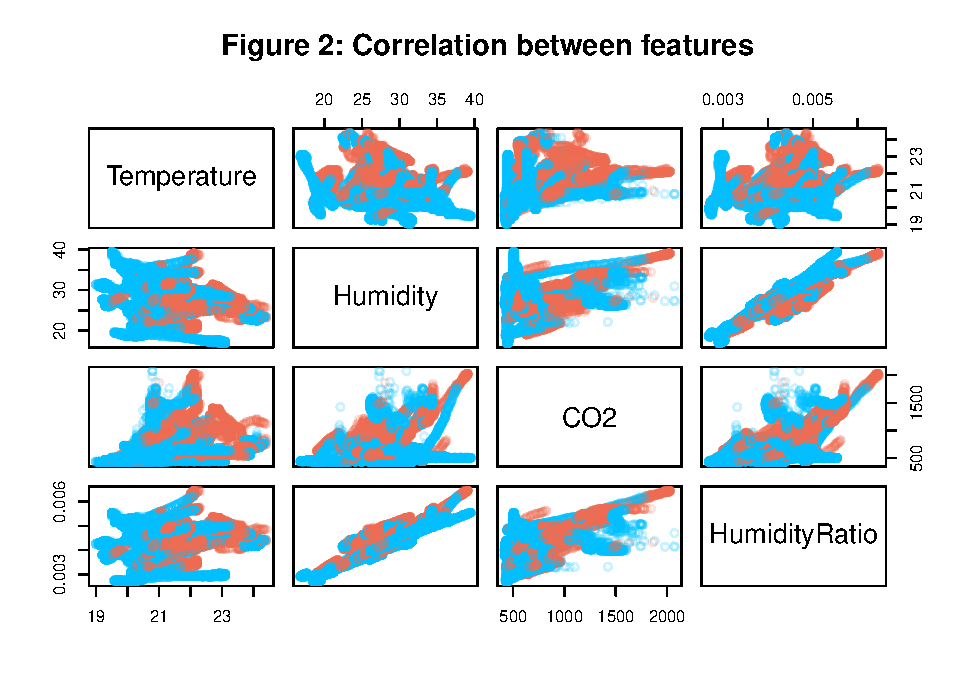
\includegraphics{Assignment-4_files/figure-latex/unnamed-chunk-3-1.pdf}

As we can see in the figure above the remaining features seem to behave
quite nicely, although some could be considered to be somewhat
correlated (e.g.~\texttt{Humidity} and \texttt{CO2}). There seem to be
some quite nice divisions of the occupancy status within the different
features which should make adequate classification quite easy.

\hypertarget{methodology}{%
\section{Methodology}\label{methodology}}

As we're dealing with a binary classification problem there are some
different methods that we've decided to test out. The methods which we
have chosen are SVM, KNN and Decision Trees. Our idea is to examine all
methods quite shallowly and then go a bit deeper for one or two that
shows promise.

\hypertarget{svm}{%
\subsection{SVM}\label{svm}}

As support vector machines are widely used in classification (SOURCE) it
seems appropriate to apply the method to this problem. In Figure 2 above
we note that we seem to have non-linear data which suggest that either a
polynomial or a radial kernel should work well, or at least better than
a linear kernel.

\hypertarget{implementation}{%
\subsubsection{Implementation}\label{implementation}}

We examine three different kernels, a linear kernel, a radial kernel as
well as a polynomial kernel. We use our aforementioned validation set in
order to perform a coarse-to-fine parameter search for the cost \(C\)
and the degree for the polynomial kernel (in the case of the polynomial
kernel we use a grid coarse grid search and then a finer search for the
best degree). Using the package \texttt{e1071} and the function
\texttt{svm} we attained the following results for the three scenarios.

For the linear kernel we only resort to a coarse parameter search as
it's performance is not going to be able to match that of the polynomial
or the radial kernel (and since the validation error is the same did not
change much over the costs examined (\(\{10^{i}\}_{i=-2}^3\)).

For the polynomial kernel we encountered some computational difficulties
when tuning our paremeters. As such we were only able to efficiently
test up until degree 3. We did note an increase in the validation
accuracy when increasing both the degree and the cost. This seems to
indicate that the data lacks a lot of noise as we seem to favor a low
bias, but high variance, classifier which we obtain by using such a high
cost.

For the radial kernel we had similar findings as we did for the
polynomial kernel. We achieved higher validation accuracies by
increasing the cost (this increase did however slow down eventually)
which prompted us to once again disregard the finer part of the
parameter search in order to simply examine higher costs.

\begin{longtable}[]{@{}lrr@{}}
\caption{SVM Test Accuracies}\tabularnewline
\toprule
Kernel & Cost & TestAccuracy\tabularnewline
\midrule
\endfirsthead
\toprule
Kernel & Cost & TestAccuracy\tabularnewline
\midrule
\endhead
Linear & 10.00 & 0.837\tabularnewline
Radial & 31622.78 & 0.915\tabularnewline
Pylynomial degree 3 & 10.00 & 0.910\tabularnewline
\bottomrule
\end{longtable}

\hypertarget{knn}{%
\subsection{KNN}\label{knn}}

As noted previously the data seems to be quite non-linear and as KNN in
a good non-linear classifier (SOURCE). As noted when examining the SVMs
in the previous section we seem to favor low bias classifiers due to an
inherent lack of noise in our data set which should inidcate that we
want a smaller \(k\). Furthermore as KNN scales well with data we should
hopefully be able to achieve quite good results given the size of our
training set (approximatley 12000 observations).

\hypertarget{implementation-1}{%
\subsubsection{Implementation}\label{implementation-1}}

Using the package \texttt{Class} and the function \texttt{knn} we do a
parameter search using our validation set for a good \(k\) on
\((1,...,50)\).

The value of \(k\) which generates the best validation accuracy turns
out to be 1. As the best kNN classifier, which performs extremely well
with a test accuracy of 0.9399319 is a 1-NN, this strongly indicates
that our data is not very noisy at all (which we also noted when
examining the SVMs).

A possible way to enhance the nearest neighbour model is through
weighting (SOURCE BOOK). A simple weighting scheme would be to weight
the k nearest neighbours by their distance to the new point we want to
classify, as such we give further emphesis to neightbours closer to the
point which we wish to classify.

In order to implement this weighting scheme we use the \texttt{kknn}
package and the included function with the same name which uses
kernel-difference weighting. The package allows for the usage of many
different kernels but the results that they produce do not differ enough
to justify an inclusion of all of them. As such we use the so called
\emph{Epanechnikov} kernel as it is one which we've encountered before.

When using weighting we actually use 25 neighbours instead of only one,
this also leads to a much higher accuracy as well at 0.9737354.

\hypertarget{decions-trees}{%
\subsection{Decions Trees}\label{decions-trees}}

Using decision trees is a good idea since we have non-linear data and a
simple binary classification problem.

\hypertarget{implementation-2}{%
\subsubsection{Implementation}\label{implementation-2}}

Constructing a simple decision tree resulted in a test accuracy of
0.9075875. This is can be further optimized by implementing bagging and
boosting algorithms.

Bagging procedures draw a predetermined number of bootstrap samples each
fitting a model. The models outputted predictions are averaged and gives
the resulting bagged estimate for each observation.

Boosting procedures train the classifier by weighting each observation
based on its classification, placing more weight on observations
incorrectly classified. The next iteration of the procedure focuses more
on those previously misclassified observations to better classify the
training data. Using the package \texttt{ipred} for bagging and the
package \texttt{adabag} for boosting we attained the following results.

\begin{longtable}[]{@{}lr@{}}
\caption{Decision Trees}\tabularnewline
\toprule
Method & Test.Accuracy\tabularnewline
\midrule
\endfirsthead
\toprule
Method & Test.Accuracy\tabularnewline
\midrule
\endhead
Simple & 0.908\tabularnewline
Bagging & 0.979\tabularnewline
Boosting & 0.955\tabularnewline
\bottomrule
\end{longtable}

In the case of bagging we draw \(1000\) bootstrap samples and in the
case of boosting we iterate over \(100\) trees. From Table 4 we can
conclude that bagging resulted in higher Test Accuracy than boosting.
Although bagging resulted in the highest Test Accuracy we loose the
interpretability of the tree based structure, since a bagged tree no
longer is a tree (The Elements of Statistical Learning, second edition,
s. 286). If interpretability is valued, the boosting procedure is worth
considering despite the lower Test Accuracy.

\hypertarget{discussion}{%
\section{Discussion}\label{discussion}}

The different methods which we've examined throughout this project yield
the following results when each of them have been tuned (although to
different degrees).

\begin{longtable}[]{@{}lr@{}}
\caption{Final Test Accuracies}\tabularnewline
\toprule
Method & Accuracy\tabularnewline
\midrule
\endfirsthead
\toprule
Method & Accuracy\tabularnewline
\midrule
\endhead
Bagging & 0.979\tabularnewline
Weighted 25-NN & 0.974\tabularnewline
Radial SVM & 0.915\tabularnewline
\bottomrule
\end{longtable}

From Table 5 we see that

\hypertarget{bibliography}{%
\section{Bibliography}\label{bibliography}}

\hypertarget{appendix}{%
\section{Appendix}\label{appendix}}

\end{document}
